% This file was created by tikzplotlib v0.9.8.
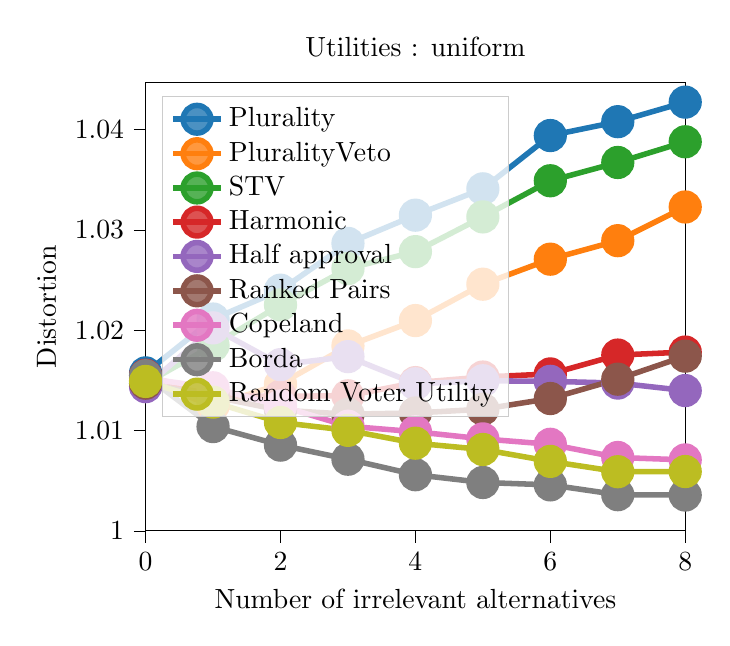
\begin{tikzpicture}

\definecolor{color0}{rgb}{0.12156862745098,0.466666666666667,0.705882352941177}
\definecolor{color1}{rgb}{1,0.498039215686275,0.0549019607843137}
\definecolor{color2}{rgb}{0.172549019607843,0.627450980392157,0.172549019607843}
\definecolor{color3}{rgb}{0.83921568627451,0.152941176470588,0.156862745098039}
\definecolor{color4}{rgb}{0.580392156862745,0.403921568627451,0.741176470588235}
\definecolor{color5}{rgb}{0.549019607843137,0.337254901960784,0.294117647058824}
\definecolor{color6}{rgb}{0.890196078431372,0.466666666666667,0.76078431372549}
\definecolor{color7}{rgb}{0.737254901960784,0.741176470588235,0.133333333333333}

\begin{axis}[
legend cell align={left},
legend style={
  fill opacity=0.8,
  draw opacity=1,
  text opacity=1,
  at={(0.03,0.97)},
  anchor=north west,
  draw=white!80!black
},
tick align=outside,
tick pos=left,
title={Utilities : uniform},
x grid style={white!69.0196078431373!black},
xlabel={Number of irrelevant alternatives},
xmin=0, xmax=8,
xtick style={color=black},
y grid style={white!69.0196078431373!black},
ylabel={Distortion},
ymin=1, ymax=1.04469602902172,
ytick style={color=black}
]
\addplot [line width=2pt, color0, mark=*, mark size=5, mark options={solid}]
table {%
0 1.01574590401617
1 1.02111285050114
2 1.0239899582187
3 1.02865447028491
4 1.03146723819318
5 1.0340927784753
6 1.03940649642039
7 1.04078974624366
8 1.04273747357987
};
\addlegendentry{Plurality}
\addplot [line width=2pt, color1, mark=*, mark size=5, mark options={solid}]
table {%
0 1.01499296366873
1 1.01246429872748
2 1.01463563050997
3 1.01843339348691
4 1.02096097586092
5 1.02458579823751
6 1.02707988385206
7 1.02892558784268
8 1.0322853777768
};
\addlegendentry{PluralityVeto}
\addplot [line width=2pt, color2, mark=*, mark size=5, mark options={solid}]
table {%
0 1.01469112503658
1 1.01848093372087
2 1.02252650185721
3 1.02614761341166
4 1.02783321878271
5 1.03129636465109
6 1.03489873671664
7 1.03672227533496
8 1.03878570667876
};
\addlegendentry{STV}
\addplot [line width=2pt, color3, mark=*, mark size=5, mark options={solid}]
table {%
0 1.01551266511878
1 1.01346909654301
2 1.01341928230423
3 1.01345919345773
4 1.01477592012681
5 1.01533010332401
6 1.01564252276817
7 1.01752257996035
8 1.01782132406558
};
\addlegendentry{Harmonic}
\addplot [line width=2pt, color4, mark=*, mark size=5, mark options={solid}]
table {%
0 1.01437034779171
1 1.02023383840785
2 1.01656960521474
3 1.0173643728812
4 1.01465385414875
5 1.01495909803544
6 1.0149028242758
7 1.01472793656746
8 1.01398159694833
};
\addlegendentry{Half approval}
\addplot [line width=2pt, color5, mark=*, mark size=5, mark options={solid}]
table {%
0 1.01471855565831
1 1.01337820676922
2 1.01202981314776
3 1.01162485558673
4 1.01174945832933
5 1.01212199448104
6 1.01318726945014
7 1.0151164992606
8 1.01741225159453
};
\addlegendentry{Ranked Pairs}
\addplot [line width=2pt, color6, mark=*, mark size=5, mark options={solid}]
table {%
0 1.01521123436056
1 1.0142589397923
2 1.01244355164651
3 1.01042602356984
4 1.00987787363902
5 1.00916518008685
6 1.00862512908933
7 1.00731025537213
8 1.00706956587249
};
\addlegendentry{Copeland}
\addplot [line width=2pt, white!49.8039215686275!black, mark=*, mark size=5, mark options={solid}]
table {%
0 1.01546380109431
1 1.01039043526382
2 1.00854002310312
3 1.00713690922691
4 1.00559118298993
5 1.0048173148388
6 1.00457778010183
7 1.00359993879336
8 1.0035663647427
};
\addlegendentry{Borda}
\addplot [line width=2pt, color7, mark=*, mark size=5, mark options={solid}]
table {%
0 1.01489204446901
1 1.0128284643381
2 1.0107995478966
3 1.01001487026379
4 1.00873573850296
5 1.00810701355302
6 1.00692112066065
7 1.00589097200685
8 1.00591043020172
};
\addlegendentry{Random Voter Utility}
\end{axis}

\end{tikzpicture}
